\section{Diagramas de conexiones}

Para la caracterización experimental y visualización del lazo de histéresis magnética en el osciloscopio, se implementa el montaje eléctrico ilustrado en la figura 5.1. Este circuito consta de una alimentación variable mediante un autotransformador (Variac) que energiza el devanado primario del transformador bajo prueba, intercalando instrumentos analógicos (amperímetro, voltímetro y wattímetro) para registrar las magnitudes eficaces y la potencia activa total absorbida por el núcleo. La señal analógica correspondiente a la intensidad de campo magnético ($H$) se obtiene directamente de la caída de tensión en la resistencia shunt ($R_s$) conectada en serie con el primario, mientras que la densidad de flujo magnético ($B$) se determina a través del voltaje integrado en el condensador de un circuito pasivo de primer orden $RC$ acoplado al devanado secundario.

 \begin{center}
        \begin{figure}[H]
        \centering  
        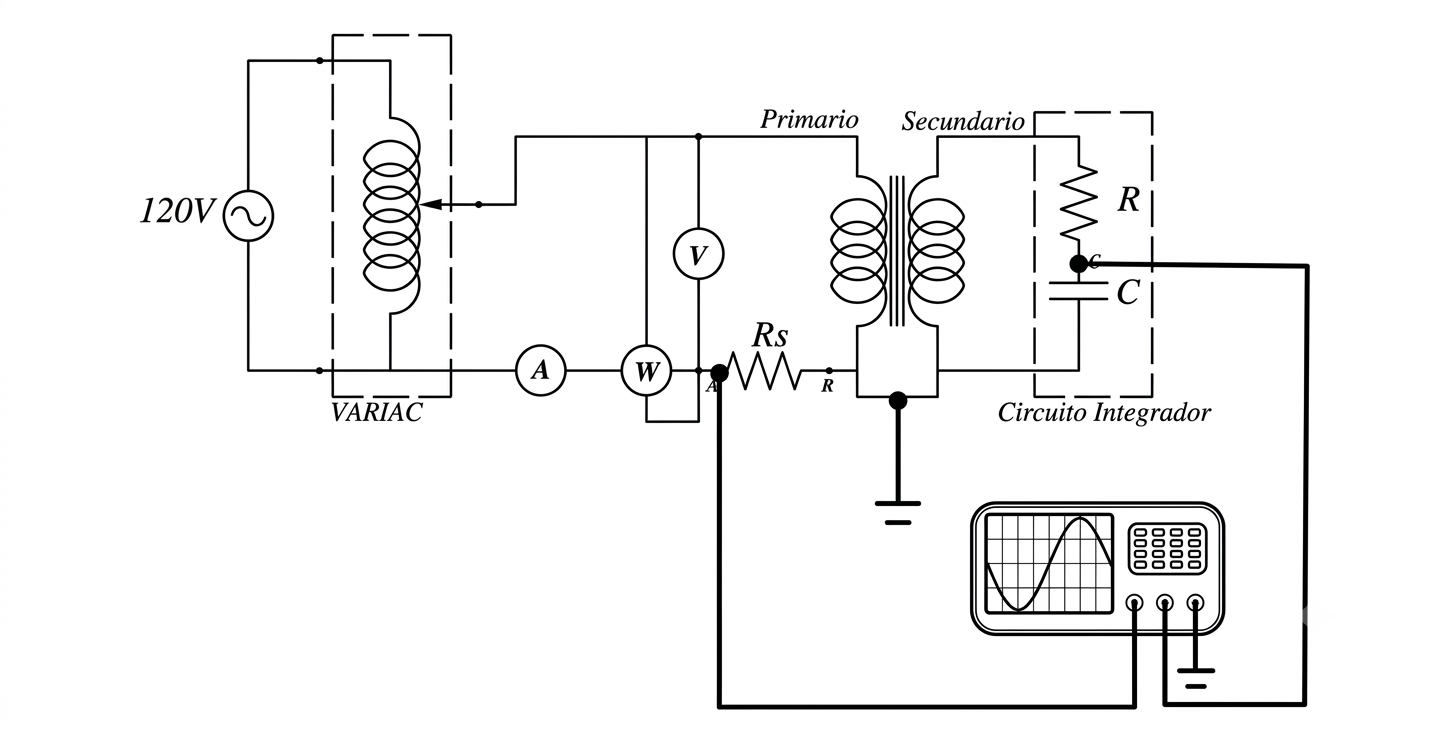
\includegraphics[scale=0.3]{imagenes/informe2.png}
        \caption{Utilización del Circuito Integrador}
        \end{figure}
    \end{center} 
        